\subsection{High-level components and their interaction}

A high-level view of the components composing the system is represented in the component diagram below [figure \ref{fig:high-lev-comp-diag}.
Each component provides an interface through which the other components can interacts with the component.
Note that not all the components represented, like the Browser, are actually components of the final system but are part of the environment with which the system will interact.

\begin{figure}[h]
	\centerline{
		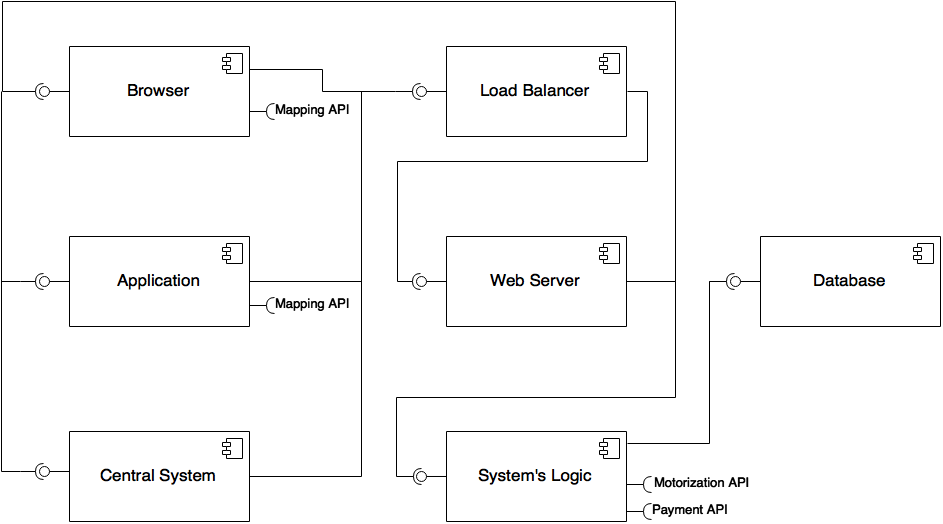
\includegraphics[width=400px]{../Datas/images/high-level-component-diagram.png}
	}
	\caption{High-level component diagram}
	\label{fig:high-lev-comp-diag}
\end{figure}

\begin{itemize}
	\item Browser: The software used by the user to access to the service.
	\item Mobile application: the application installed on mobile devices and used by the user to access to the service.
	\item Central system: also called Car's Central System. It's the software responsible for car's management and interfacing with the System.
	\item Load balancer: the software used to distribute the workload to the servers.
	\item Web server: the software used to elaborate requests and sends back responses.
	\item System's logic: the software responsible for the whole systemìs logic.
	\item Database: the software unit responsible for the management of queries and data.
\end{itemize}
